\section{Building a Quadtree}
\textbf{Download a file containing 1200 particle masses and positions, the data is in group /PartType4. Considering only the x and y coordinates of these particles (between 0 and 150), construct a quadtree with at most 12 particles per leaf node. You can treat the masses and positions as dimensionless and use G=1. You are free to use the where function and/or masks. Plot the particles and indicate which particles are in which node. Calculate the n=0 multipole moment for the leaf node containing the particle with index i=100 and that of all of its parent nodes up to and including the root node.}


The setup of the Quad Tree implementation in Python uses three classes: \textit{Point}, \textit{Node} and \textit{QuadTree}. This setup is inspired from the following blogpost: \url{https://kpully.github.io/Quadtrees/} and works very intuitively.
The \textit{Point} is simply a class that stores the $x$ and $y$ position of a point. The \textit{Node} is a class that contains points and may contain (4 in 2D) children (which are also nodes). The \textit{QuadTree} class then contains the points and nodes, and a method to subdivide the root-node, which initially contains all points, into multiple nodes which contain only some threshold amount of points.

The code that generates the tree, subdivides the root-node into children, calculates the multipole moments and finds the parents of some leafnode that contains a certain point is given below.

\lstinputlisting[]{question7.py}

This script produces the following outputs:
\lstinputlisting[language={}]{q7output.txt}

The script produces Figure \ref{fig:fig60} that shows the boxes defined by the leaf nodes. The boxes contain at most 12 particles. As can be seen from the output of the script, the root-node has a multipole moment of 1200, which verifies that the multipole moment calculation is working, since there are 1200 particles with unit mass, so the multipole moment of the root-node is expected to be 1200.

\begin{figure}[ht]\centering
\centering
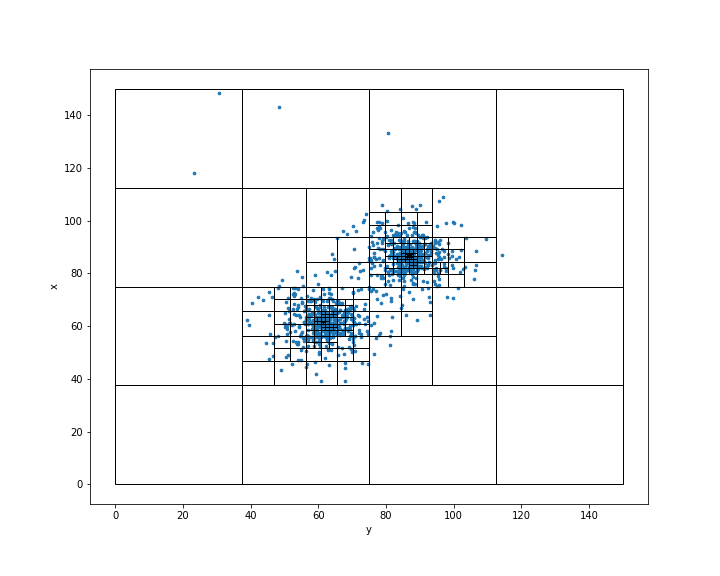
\includegraphics[width=0.8\linewidth]{./plots/q7_1.pdf}
\captionsetup{width=0.8\linewidth}
\captionof{figure}{Quad tree of the 1200 points. The leaf nodes are shown as boxes that contain at most 12 points.}
\label{fig:fig60}
\end{figure}


